%\documentclass{article}
%\documentclass[10pt,a4paper]{report}
%\usepackage{amsmath}
%\usepackage{amssymb}
%\usepackage{gensymb}
%\usepackage{amsfonts}
%\usepackage{setspace}
%\usepackage{tasks}
%\usepackage{graphicx}
%\usepackage{float}
%\usepackage{listings}
%\newcommand{\myvec}[1]{\ensuremath{\begin{pmatrix}#1\end{pmatrix}}}
%\let\vec\mathbf
%\providecommand{\sbrak}[1]{\ensuremath{{}\left[#1\right]}}
%\providecommand{\lsbrak}[1]{\ensuremath{{}\left[#1\right.}}
%\providecommand{\rsbrak}[1]{\ensuremath{{}\left.#1\right]}}
%\providecommand{\brak}[1]{\ensuremath{\left(#1\right)}}
%\providecommand{\lbrak}[1]{\ensuremath{\left(#1\right.}}
%\providecommand{\rbrak}[1]{\ensuremath{\left.#1\right)}}
%\providecommand{\cbrak}[1]{\ensuremath{\left\{#1\right\}}}
%\providecommand{\lcbrak}[1]{\ensuremath{\left\{#1\right.}}
%\providecommand{\rcbrak}[1]{\ensuremath{\left.#1\right\}}}
%\providecommand{\norm}[1]{\left\lVert#1\right\rVert}
%\providecommand{\abs}[1]{\left\vert#1\right\vert}
%\let\vec\mathbf
%\newcommand{\norm}[1]{\lVert#1\rVert}
%\renewcommand{\vec}[1]{\textbf{#1}}
%\begin{document}
%\onehalfspacing
%\begin{center}
%	\section*{\textbf{Class 11}}
%	\subsection*{Chapter 10 - STRAIGHT LINES}
%\end{center}
%The following problem is question 11 from exercise 10.4
%\begin{enumerate}
 %   \item Find the equation of the lines through the point (3, 2) which make an angle of 45\degree  with the line x – 2y = 3.
%\end{enumerate}
%\textbf{Solution:}\\
The given line parameters are
\begin{align}
   \vec{n}=\myvec{1\\-2},c=-5\\
	\vec{P}=\myvec{3\\2}
\end{align}
yielding
\begin{align}
\vec{m}_1=\myvec{2\\1}\\
\vec{m}_2=\myvec{1\\m}
\end{align}
where  $m$ is defined to be the slope of the line. If the angle between the lines be $\theta$,

\begin{align}
\cos \theta = \frac{\vec{m}_1^\top \vec{m}_2}{\norm{\vec{m}_1}\norm{\vec{m}_2}}\\
	\text{given, } \theta = 45\degree\\
\implies \cos45\degree =  \frac{\vec{m}_1^\top \vec{m}_2}{\norm{\vec{m}_1}\norm{\vec{m}_2}}\\
\implies \frac{1}{\sqrt{2}} = \frac{\myvec{2 & 1} \myvec{1\\m}}{\norm{\myvec{2\\1}}\norm{\myvec{1\\m}}}
\end{align}
\begin{align}
\implies \frac{1}{\sqrt{2}}=\frac{2+m}{\sqrt{2^2 + 1}\sqrt{m^2 + 1}}\\
\implies \frac{1}{2}=\frac{m^2 + 4m +4}{5m^2 +5}\\
\text{or, } 3m^2 - 8m -3 = 0
\end{align}
yielding
\begin{align}
m= - \frac{1}{3}, 3
\end{align} 
when m=3,the equation of line passing through $\vec{P}$  is then obtained as
\begin{align}
\vec{n}^{\top} ({\vec{x}-\vec{P}}) = 0\\
\text{where,}{\vec{n}}=\myvec{m\\-1} \\
{\vec{n}}=\myvec{3\\-1} \\
\implies 
	\myvec{3&-1}\cbrak{\vec{x}-\myvec{3\\2}}&=0\\
	&=7 \\
 \implies 	\myvec{3 & -1}\vec{x} &= 7
\end{align}
And, when $m=-\frac{1}{3}$,the equation of the line passing through $\vec{P}$  and having a slope of $-\frac{1}{3}$is
\begin{align}
\vec{n}^{\top} ({\vec{x}-\vec{P}}) = 0\\
{\vec{n}}=\myvec{-\frac{1}{3}\\-1} \\
\implies {\vec{n}}=\myvec{1\\3} \\
\implies 
	\myvec{1&3}\cbrak{\vec{x}-\myvec{3\\2}}&=0\\
	&=9 \\
		\implies 	\myvec{1 & 3}\vec{x} &= 9
\end{align}
Therefore,the equations of the lines are 
\begin{align}
	\myvec{3 & -1}\vec{x} = 7  \text{ and }   \myvec{1 & 3}\vec{x} = 9 .
\end{align}
%\begin{figure}[H]
%\centering
%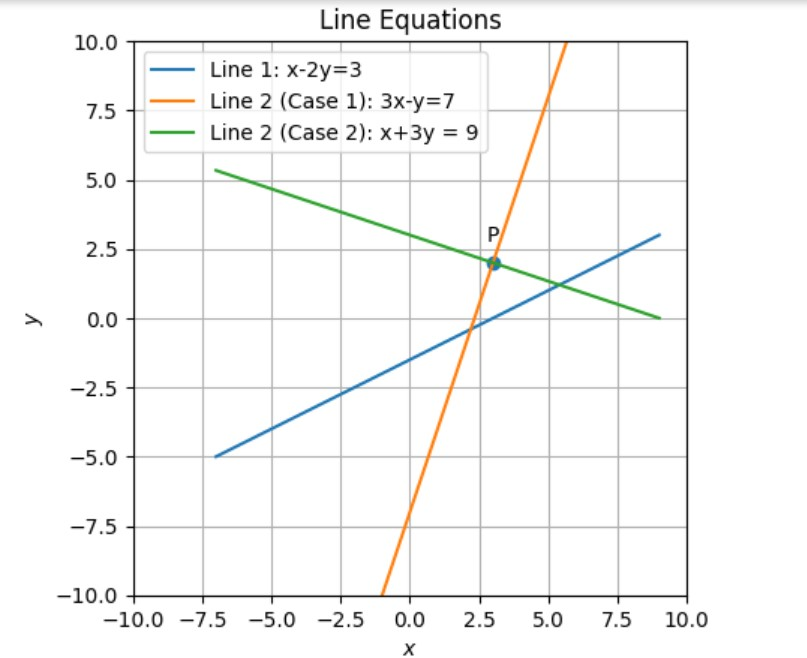
\includegraphics[width=\columnwidth]{figs/strline.jpg}
%\caption{STRAIGHT LINES}
%\label{fig:strline.jpg}
%\end{figure}




%\end{document}
